\section{N-grams}
\begin{frame}{}
    \LARGE Natural Language Processing: \textbf{N-grams}
\end{frame}

\begin{frame}{What are N-grams?}
    \begin{figure}
        \centering
        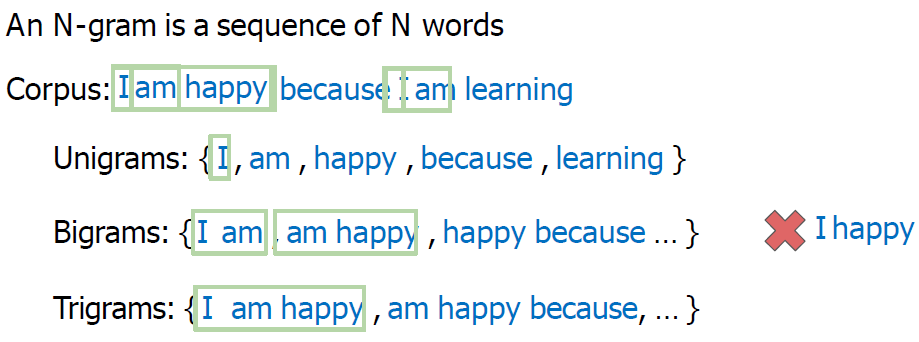
\includegraphics[width=\textwidth,height=0.8\textheight,keepaspectratio]{images/nlp-intro/ngram.png}
    \end{figure}
    \vspace{1em}
    \begin{itemize} 
        \item Items are typically \textbf{words} or \textbf{characters}.
    \end{itemize}
\end{frame}

\begin{frame}{Tokenization}
    \begin{itemize}
        \item Tokenization is the process of breaking text into smaller units called \textbf{tokens}.
        \item Tokens can be words, characters, or subwords.
        \item Example: "I love NLP" can be tokenized into:
        \begin{itemize}
            \item Words: ["I", "love", "NLP"]
            \item Characters: ["I", " ", "l", "o", "v", "e", " ", "N", "L", "P"]
            \item Subwords: ["I", " ", "lov", "e", " ", "N", "L", "P"]
        \end{itemize}
        \item Tokenization is crucial for preparing text data for NLP tasks.
    \end{itemize}
\end{frame}

\begin{frame}{Examples of N-grams}
    \textbf{Sentence:} ``I love NLP''

    \vspace{1em}
    \begin{itemize}
        \item \textbf{Unigrams:} I,\ love,\ NLP
        \item \textbf{Bigrams:} I\ love,\ love\ NLP
        \item \textbf{Trigrams:} I\ love\ NLP
    \end{itemize}
\end{frame}

\begin{frame}{Why Use N-grams?}
    \begin{itemize}
        \item Capture local word co-occurrence
        \item Build simple language models
        \item Easy to compute and analyze
        \item Trade-off between simplicity (unigram) and contextual richness (trigram)
    \end{itemize}
\end{frame}
